\documentclass[12pt,a4paper,utf8x]{report}



%%%%%%%%%%%%%%%%%%%%%%%%%%%%%
%         MODULES           %
%%%%%%%%%%%%%%%%%%%%%%%%%%%%%

\usepackage[english]{babel}
\usepackage{ucs}
\usepackage[utf8x]{inputenc}
\usepackage{url}				% URL
\usepackage{geometry}			% Marges
\usepackage{graphicx}			% Images
\usepackage{listings}			% Code source
\usepackage{lscape}				% Mode paysage
\usepackage{multicol}			% Colonnes
\usepackage{makeidx}			% Indexation
\usepackage{setspace}			% Interlignage
\usepackage[dvipsnames]{xcolor}
\usepackage{caption}
\usepackage{appendix}
\usepackage{nameref} 



%%%%%%%%%%%%%%%%%%%%%%%%%%%%%
%         SETTINGS          %
%%%%%%%%%%%%%%%%%%%%%%%%%%%%%

\makeindex
\definecolor{codegray}{rgb}{0.9,0.9,0.9}
\geometry{a4paper, top=2.5cm, bottom=3.5cm, left=1.5cm, right=1.5cm, marginparwidth=1.2cm}		% Marges
\parskip=5pt 																					% Espaces paragraphes
\sloppy																							% Marge à droite
\setlength{\parindent}{15mm}																	% Indentation
\setlength{\itemsep}{0pt}
\interfootnotelinepenalty=150
\widowpenalty=150
\clubpenalty=150 
\lstset
{
	language=C,
	tabsize=3,
	frame=lines,
	keywordstyle=\color{blue},
	commentstyle=\color{OliveGreen},
	stringstyle=\color{red},
	numbers=left,
	numberstyle=\tiny,numbersep=5pt,breaklines=true,showstringspaces=false,basicstyle=\footnotesize,emph={label},
	backgroundcolor=\color{codegray},
}
\newlength{\wideitemsep}
\setlength{\wideitemsep}{\itemsep}
\addtolength{\wideitemsep}{-5pt}
\let\olditem\item
\renewcommand{\item}{\setlength{\itemsep}{\wideitemsep}\olditem}



%%%%%%%%%%%%%%%%%%%%%%%%%%%%%
%          MACROS           %
%%%%%%%%%%%%%%%%%%%%%%%%%%%%%

\newcounter{iannexe}
\newcommand{\othertitle}[1]
{
	\vspace*{1.5cm}
	\hspace*{-1.5cm}{\huge \textbf{#1}}
	\vspace{1.5cm}
}

\newcommand{\cfunction}[1]
{
	{\fontfamily{lmtt}\selectfont #1}
}

\newcommand{\console}[1]
{
	\colorbox{black}{\begin{minipage}[c]{1\linewidth}\textcolor{white}{\texttt{#1}}\end{minipage}}
}


% Enlever le nom chapitre
\makeatletter
\def\@makechapterhead#1{%
  \vspace*{50\p@}%
  {\parindent \z@ \raggedright \normalfont
    \interlinepenalty\@M
    \ifnum \c@secnumdepth >\m@ne
        \Huge\bfseries \thechapter\quad
    \fi
    \Huge \bfseries #1\par\nobreak
    \vskip 40\p@
  }}

\def\@makeschapterhead#1{%
  \vspace*{50\p@}%
  {\parindent \z@ \raggedright
    \normalfont
    \interlinepenalty\@M
    \Huge \bfseries  #1\par\nobreak
    \vskip 40\p@
  }}
  
\def\@part[#1]#2{%
    \ifnum \c@secnumdepth >\m@ne
      \refstepcounter{part}%
      \addcontentsline{toc}{part}{\thepart\hspace{1em}#1}%
    \else
      \addcontentsline{toc}{part}{#1}%
    \fi
    \vspace*{50\p@}%
    {\huge\bfseries #2}%
    \nobreak
    \vskip 3ex
    \@afterheading}  
  
\makeatother



%%%%%%%%%%%%%%%%%%%%%%%%%%%%%
%           BODY            %
%%%%%%%%%%%%%%%%%%%%%%%%%%%%%

%% Couverture
\title
{
	\normalsize
	{
		Teesside University\\
		School of Computing\\
		2011 - 2012\\
	}
	\vspace{45mm}
	\textbf{Final Year Project}\\
	\normalsize{BSc Computer Science}\\
	\vspace{10mm}
	\huge{Social network library development}\\
}

\author
{
	Thibaut Havel\\
	\normalsize{L1247434}\\
	\vspace{45mm}
}

\date
{
	\normalsize
	{
		Supervisor: Jo\~{a}o F. Ferreira\\
		Second reader: Erika Downs
	}
}


%% Pages
\begin{document}
\maketitle
\begin{onehalfspace}
\part{Abstract}

The main aim of this project is to develop a low-level library that is able to grab and store data from a social network. This library works in an embedded device and stored data had to be used to provide a simple service. To demonstrate the effectiveness of the final library, I created a demo service that interacts with a known social network (for example, Twitter).

% FreeRTOS

% To write at the end


\clearpage

\chapter*{Acknowledgements}

\hspace{15mm}I would like to thank my supervisor Jo\~{a}o Ferreira for his support all over the development of my project.


\clearpage
\tableofcontents
\chapter{Introduction}

\hspace{15mm}Our society tends to use more and more social networks (for instance, Twitter or Facebook). At the same time, we are increasingly dependent on the use of embedded devices on a day-to-day basis (for instance, home automation). The goal of this project is to develop a software platform that allows an effective and efficient communication between embedded devices and social networks.

The main aim is to develop a low-level library that is able to grab and store data from a social network. This library was designed for embedded devices and allows data to be stored and to be used to provide a simple service. To demonstrate the effectiveness of the final library, I created a demo service that interacts with a known social network: Twitter.

One of my personal objectives was to improve my knowledge in low-level development and become familiar with the C language. Also I was looking forward to improving my software development skill while working with a very specific hardware.

Firstly, this report will present the way I started my initial research and how I designed the library according to my functional choices. Secondly, it will present how I've implemented these functionalities, and what I did to test my library. Finally, this report will end by an evaluation of the final product regarding the design choices, the way I've implemented them, and his reliability.


\clearpage

\chapter{Methodology}

%---------------------------------------------------------------
\section{The initial project scheduling}

\hspace{15mm}In my project specification, I set my schedule as following:
\begin{itemize}
\item January: Research (2 weeks), design (2 weeks).
\item Febuary: Design (1 week), Implementation (3 weeks).
\item March: Implementation (3 weeks), Testing (1 week).
\item April: Evaluation and report compilation (2 weeks).
\end{itemize}

My supervisor Jo\~{a}o and I met every week or every two weeks to discuss about the planning and progresses of my project. 


%---------------------------------------------------------------
\section{Research plan}

\hspace{15mm}My initial approach was to become familiar with the embedded device technology. I had to find an adapted, small and simple operating system to work with, thereby I chose \textbf{FreeRTOS}\footnote{FreeRTOS is a light-weight Real-Time Operating System.} supported from my supervisor.

He had already used this system and he had developed applications before. He provided me one of his own device running with FreeRTOS. So, thanks to Jo\~{a}o and his knowledge about this operating system, I had a platform in addition to a massive support from him and the online community to develop my library. As I didn't have any knowledge about FreeRTOS, I read several articles which deals with how it works, and how tasks are scheduled in an real-time way.

As a consequence of this choice and because one the goals of this project is to gain knowledge about low-level development, the library was built using the C language.

Then, I defined every functionality of the final applications. Basically, the library's features are simple: it should allow a user to receive and send text from and to a social network. For instance a \textit{message on the wall} in \textbf{Facebook} or a \textit{tweet} in \textbf{Twitter}. Facebook and Twitter are both well known social networks and after some research about them, I choose to build my library suitable for Twitter because of the solid support for \textbf{OAuth} which is a secured protocol to access data. Once again, this choice was supported by Jo\~{a}o.

At this point, I had to define how to receive and send tweets, so I've started by looking for any existing solutions. In the next chapter, I will discuss why I chose to build my own library from scratch only using OAuth.

After this key decision, I've learned how OAuth works and how to register an application on Twitter in order to access to the data.

As I was now aware about what the tools I will be using and the way to use them, I designed the library according to the features I wanted to implement.

The next step of the development was to implement the abstract structure of the library. At this stage, I faced lot of issues concerning the use of OAuth, the C language and its requirements. During my previous years of studies I learnt the basics of this language but to build the library I had to read a lot of articles, books and tutorials along the implementation.

Once I had finished the draft version of the library, I tested every functionality by receiving and sending tweets over my own account and I improved the reliability according to the results of these tests.

% If enought time left : fit this with existing method


%---------------------------------------------------------------
\section{The support tools}

\hspace{15mm}To help myself into the research and the development of the library, I used some additional appropriate tools:
\begin{itemize}
\item A diary: to keep every relevant informations but also as a memory trail of the development chronology.
\item Github\footnote{Github is an online project hosting.}: to back up the source code and share my progress with my supervisor.
\item FreeRTOS POSIX\footnote{Standards to maintaining compatibility between UNIX operating systems.} simulator: to develop and to test my library without any embedded device.
\end{itemize}

\clearpage

\chapter{Research}\label{chap:research}

%---------------------------------------------------------------
\section{Operating System: FreeRTOS}

\subsection{Overview}

(Quick overview of the system: Free, open source, GP Licence, light-weight)


\subsection{Real-Time System}

(Kernel mechanism: priorities and scheduling)


\subsection{Libraries}

(Existing libraries: non-free libraries for specific hardware, light system library)


\subsection{POSIX simulator}

(Compilation of a library and a task)



%---------------------------------------------------------------
\section{Twitter authentication: OAuth protocol}

\subsection{Overview}

(Common authentication mechanism: token, secret key system, include graphic representations)


\subsection{Existing library in C}

(Downloaded and tested library: samples hard to understand, idea: create a simple-to-use library layer)


\subsection{Register an application on Twitter}

(Way and proprieties of the registered application)


\subsection{Required libraries}

(libcurl: overview and it's seem hard to adapt to FreeRTOS, idea: create a very simple HTTP request library)\\
(OpenSSL: overview and it's seem hard to adapt to FreeRTOS, idea)



\clearpage
\chapter{Design of the library}


%---------------------------------------------------------------
\section{Functional design}

\subsection{Interactions with Twitter}

\hspace{15mm}Basically, the final library should enables a developer:
\begin{itemize}
\item To authenticate its application to Twitter. 
\item To send tweets to Twitter.
\item To receive tweets from Twitter.
\end{itemize}

And these features have to work whatever the operating system and the hardware architecture.

I chose not implement any storing properties because it is more flexible to let the developer chose the way he wants to store tweets.


\subsection{A user-friendly layer}

\hspace{15mm}This library has to be a user-friendly layer. The developer does not have to know how OAuth works to build its own application to access to Twitter. He just have to give the basic informations about the registered application (the public and secret key provided by Twitter) and informations about its Twitter account (the login and password).

The first main functionality is the authentication process which gathers all OAuth operations and returns an authentication entity (for instance, typed as a C structure) which could be use by the developer in a further step to send and to receive tweets. This entity contains every required informations needed to allow OAuth to connect to Twitter. 

The send functionality is one of the two behaviours which could use the authentication entity in order to send a tweet on a Twitter profile.

Finally, the receive functionality use the authentication entity as well in order to receive tweets from a Twitter account's \textbf{timeline}\footnote{The timeline is the part of a Twitter profile which contains all tweets sent by a user.}. This functionality include parsing functions which enables to return a set of tweets entities. 
% To be developed

Each functionality is represented by a single function. Nevertheless, the content of a functionality could be split into several operation each represented by another function.



%---------------------------------------------------------------
\section{Implementation design}


\subsection{Functions implementations}

% Describe relevant behaviours of each functionalities:
% - Authentication using OAuth HTTP post/get.
% - Send tweet using the authentication structure.
% - Receiving tweet using my own parsing functions, etc.

\hspace{15mm}Every steps of the authentication process are gather into the main authentication function. Basically each use of the OAuth library for a specific stage of the synchronisation is surrounded by a set of operations, for this very reason each stage is defined into a distinctive function. As explained above in the chapter \nameref{chap:research}, to authenticate an application to Twitter and then be able to access to the timeline or to send a tweet is simple but it requires few steps:
\begin{itemize}
\item 1- Consumer token: it is the first token given by the Twitter service provider.
\item 2- Request token: it requests the token needed to obtain user authorization.
\item 3- Verifier: it uses the request token in order to get the PIN code (or verifier). 
\item 4- Access token: it uses the verifier to request the final token which will be use to send or receive tweets.
\end{itemize}
This main function gives to the user an authentication entity, that is the one he provides to the behaviour functions (send and receive). This entity is typed as a C structure.

As every behaviour functions, the send function need the access token to be able to send a text message over Twitter. The main function retrieves the needed informations from the authentication entity which are given as parameters in sub-functions\footnote{A sub-function is used by the main function in a distributed way to perform the goal.}. Whatever the sub-function, no field of the authentication entity is directly used, only the main function holds this responsibility.

To get the tweets from the user's timeline, a request is firstly send to the Twitter service provider. The result is a XML content which is parsed by some sub-functions. These parsing functions determine how many tweets are there in the timeline, and for each of them a new structure is created. Thus, the main function gives to the developer a collection of tweets each represented by a C structure which contains the most significant informations about it (e.g. the date, the text content).


\subsection{Functional diagram of the library}

% - UML-like representation of the way it will work

\begin{figure}[h]
  \centering
  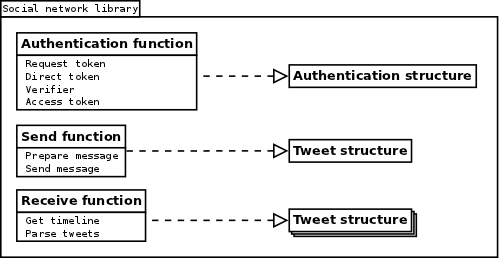
\includegraphics[scale=0.75]{images/functional_design.png}
  \caption{Functional diagram representing the implemented design}
\end{figure}


\clearpage
\chapter{Implementation}

%---------------------------------------------------------------
\section{Required libraries}

\hspace{15mm}To be able to write the library, I first decided to implement the dependencies: \textit{liboauth}, \textit{OpenSSL} and \textit{libcurl}.

I started by downloading liboauth. The content of the library is really simple because it consists of eight C source code and header files. I managed to compile the FreeRTOS simulator including the OAuth library: in order to do so, I first edited the simulator \textit{makefile}\footnote{A makefile is a file containing compilation instructions.} by hand.

\begin{figure}[h]
  \centering
  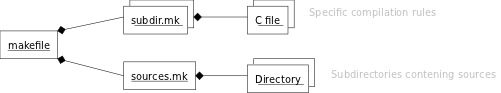
\includegraphics[scale=0.75]{images/makefile.png}
  \caption{FreeRTOS POSIX simulator, makefile architecture}
\end{figure}

As shown in the figure above, the compilation instructions are gather into a \textit{Debug} folder where rules are split into sub-files. Thus, I added a \textit{subdir.mk} listing the C source codes files of the library and I referenced the name of the sub-directory into \textit{sources.mk}.

To compile liboauth the system requires \textit{OpenSSL} and \textit{libcurl}. Therefore I added some GCC options that references these libraries into the makefile: \textit{-lssl -lcrypto -lcurl}. Nevertheless, the libraries used are those installed on my own system, not those specific to simulated FreeRTOS system, which is not suitable for an embedded environment.

The best possibility could be to port OpenSSL and libcurl to FreeRTOS in order to make liboauth totally independent of my system. These libraries are massive and require many research to be ported, moreover that was not an immediate priority under the plan, so I chose to set aside this issue until my Twitter library works.


%---------------------------------------------------------------
\section{Authentication process}

\hspace{15mm}Prior to determining the authentication process, I defined the required informations to perform it as follows:
\begin{itemize}
\item The \textit{Consumer token} allows a specific application to access data from Twitter.
\item The user login and password prove this user allows the application to access to his timeline.
\item The URL to send requests are static informations given by Twitter.
\end{itemize}
I chose to defined the \textit{Consumer token} and the user informations as parameters of the main authentication function. In this way, the developer will be able to chose which Twitter application and which Twitter account would used by the library to access data. The URL are defined as static fields into the library.

Then, the first step of the authentication is the use of the \textit{Consumer token} given by Twitter to get the \textit{Request token}. Whatever the request, the URL and sometimes the parameters are generated into a specific function according to the Twitter specifications. For this first stage:
\begin{lstlisting}
twitter_request_token_url(consumer_key, consumer_secret, &request_token_url);
twitter_request_token(request_token_url, &request_token_key, &request_token_secret, &callback);
\end{lstlisting}
Basically, the output parameters begin by the \cfunction{\&} symbol because I assign the result values to the specified variables, so I need to know its references.
For instance, the first function use the \cfunction{consumer\_key} and the \cfunction{consumer\_secret} to get the generated \cfunction{request\_token\_url}. And the second one use the \cfunction{request\_token\_url} value to return the \cfunction{request\_token\_key}, the \cfunction{request\_token\_secret} and the \cfunction{callback}.

The \textit{Verifier} step is probably the most important but also the more complex. As usual, the URL is generated by a function and then the request is sent by another one:
\begin{lstlisting}
twitter_direct_token_url(request_token_key, &direct_token_url);
twitter_verifier(direct_token_url, request_token_key, &verifier);
\end{lstlisting}
But the \cfunction{twitter\_verifier} function is divided into several steps:
\begin{itemize}
\item Send a HTTP GET request using OAuth: \cfunction{oauth\_http\_get()}.
\item Parse the HTML result of the request and get the authenticity code using \cfunction{twitter\_direct\_token\_authenticity()}.
\item Regenerate another URL and some parameters using the authenticity code, and the user account informations through \cfunction{twitter\_direct\_token\_url2()}.
\item Send a HTTP POST request using the OAuth with the new URL and the generated parameters: \cfunction{oauth\_http\_post()}.
\item Parse the HTML result of the request and get the final PIN code (or verifier) with \cfunction{twitter\_direct\_token\_pin()}.
\end{itemize}

The final step of the authentication is to obtaining the \textit{Access token}:
\begin{lstlisting}
twitter_access_token_url(consumer_key, consumer_secret, request_token_key, request_token_secret, verifier, &access_token_url);
twitter_access_token(access_token_url, &access_token_key, &access_token_secret, &access_token_user_name, &access_token_user_id);
\end{lstlisting}
These functions use the two first tokens (\textit{Consumer} and \textit{Request}) and the \textit{Verifier} to obtain the final token which could be use as a proof of user authenticity and user allowance about data accessing from his timeline.

Finally, the main function gives to the developer a C entity (typed as a structure) called \cfunction{twitterAuthEntity} and defined with the following fields:
\begin{itemize}
\item The user identifier and screen name.
\item The \textit{Consumer token} key and secret.
\item The \textit{Access token} key and secret.
\end{itemize}


%---------------------------------------------------------------
\section{Send a tweet}

\hspace{15mm}As all operations allowed by the final library, the main function require the authentication entity. Thus, this entity is one of the parameter and the fields of the structure which store the details of the authentication are used inside the function in order to perform the send operation.

The second parameter is the content of the tweet, indeed. Twitter allows to send text-based posts of up 140 characters. Other extra-details might be attached to the tweet (e.g. the geo-localisation) but this library only supports the text content.

To perform the submission, the library first generate the URL and the parameters of the HTTP POST request, and then send the tweet:
\begin{lstlisting}
twitter_tweet_url(tweet_content, consumer_key, consumer_secret, access_token_key, access_token_secret, &tweet_url, &tweet_param);
twitter_tweet(tweet_url, tweet_param, &post_result);
\end{lstlisting}

If the last function succeed, it gives the XML value of the submitted tweet. This content is parsed and returned as a \cfunction{tweet} which is typed as a structure with the following fields:
\begin{itemize}
\item The tweet identifier.
\item The creation date.
\item The user screen name.
\item The tweet text content.
\end{itemize}


%---------------------------------------------------------------
\section{Receive a tweet}

\hspace{15mm}The main function gets the entire timeline which means all tweets are received using one routine:
\begin{lstlisting}
twitter_timeline_user(consumer_key, consumer_secret, access_token_key, access_token_secret, access_token_user_name, &timeline_user);
\end{lstlisting}

The received content is in XML format and the data structure is defined as follows:

\begin{figure}[h]
  \centering
  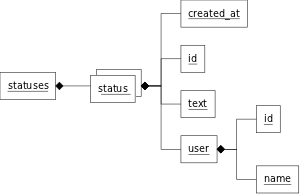
\includegraphics[scale=0.75]{images/xml.png}
  \caption{Tweets XML data structure}
\end{figure}
In the figure above, I chose to display only useful elements of the structure: those I use to fulfil \cfunction{tweet} entities.

To parse XML data I written some tool functions to count, give a value or all values from specific elements:
\begin{lstlisting}
char * xml_parser_get (const char * xml_content, const char * element_key)
int xml_parser_count (const char * xml_content, const char * element_key)
void xml_parser_getall (const char * xml_content, const char * element_key, char * element_value[])
\end{lstlisting}

Using these functions, the main one enables the developer to get an array of \cfunction{tweet}.

\clearpage
\chapter{Testing of the library}


%---------------------------------------------------------------
\section{FreeRTOS POSIX simulator}

\hspace{15mm}To test my library, I used the FreeRTOS POSIX simulator running on my Linux operating system. I first created a simple task executing step by step the authentication process and using the standard output to be sure everything works. First of all, I did not use the three main functions (authentication, send and receive) to perform my initial tests.

To compile the simulator including the demo task and the libraries and to execute it:
\begin{lstlisting}
cd FreeRTOS_Posix/Debug/
make clean; make all
./FreeRTOS_Posix
\end{lstlisting}

This task used static fields containing the required informations to proceed the authentication: the \textit{Consumer token} provided by Twitter and the details of my personal account. For each step, I chose to display the content of the returned values in order to be sure that the operations are successful done.

For instance, the output console displays for first steps of the authentication:
\begin{lstlisting}
Step 1 --------------------------------
request_token_url : https://api.twitter.com/oauth/request_token?oauth_consumer_key=VB5FifD1HLhmLmsj8tZA&oauth_nonce=b7D1myYQGy_yF_5RFrLs0&oauth_signature_method=HMAC-SHA1&oauth_timestamp=1334924651&oauth_version=1.0&oauth_signature=rGoA99tkEd%2B7%2F2RpSvZOzm%2FqVWI%3D 

Step 2 --------------------------------
request_token_key    : ebvnwX6MslItt3uPwzXxN6TcNdbzy3Q9byZN0cr0Dwc 
request_token_secret : tEcLdyfssLstUOWgvm9of3sBrjakqIGTaGrbWr0A8cs 
callback             : true 
\end{lstlisting}

The \textit{receive tweet} request displayed the whole XML content, so I chose to redirect the standard output to a temporary file. For instance, a tweet was first displayed as follows:\clearpage
\begin{lstlisting}
<status>
  <created_at>Tue Apr 03 16:23:32 +0000 2012</created_at>
  <id>187213757825564672</id>
  <text>Multi-tweets test.</text>
  // irrelevant elements
  <user>
    <id>488884688</id>
    <screen_name>thibaut_havel</screen_name>
    // irrelevant elements
  </user>
</status>
\end{lstlisting}

Then, I tested the main functions using the resulted entities (\cfunction{twitterAuthEntity} and \cfunction{tweet}) and tried to make it crash: for instance, by specifying wrong parameters.

As I wrote in the previous chapter, I have added some referencing options to the GCC compiler to be able to use liboauth in my library, thus the simulator used the dependencies installed on my own system because I did not ported them. However, except the issue of these portable libraries (OpenSSL and libcurl), my project has been running successfully on the simulator, which means that the library is also portable and it has been supposed to work on an embedded device using FreeRTOS as operating system.


%---------------------------------------------------------------
\section{Embedded device }

\hspace{15mm}The week before the deadline, Jo\~{a}o and I tried to set up the library in the embedded device using the compiler specific to the micro-controller. But we did not manage to do that because of the two dependencies that I decided to put aside and to port only if I had enough time left, which did not happen.

Nevertheless, as I wrote above, this issue does not mean that the library is not portable.



\clearpage
\chapter{Evaluation of the ptoject}


%---------------------------------------------------------------
\section{Goal}

(Is my goal achieved, why/why not?)\\
(Is my work could be use by someone else, why/why not?)


%---------------------------------------------------------------
\section{Schedule}

(Did I follow my schedule, why/why not?)


%---------------------------------------------------------------
\section{Improvements}

(What is it possible to do to improve my library?)



\clearpage

\chapter{Conclusion}

\hspace{15mm}In this final year project, I have presented the development of a social network library written in a low-level language. This library enables a developer to authenticate his application on \textbf{Twitter}, but also to receive and send text-based messages called \textit{tweets}.

This features has been tested on the simulator of a lightweight operating system: \textbf{FreeRTOS}, which proves the portability and the partial independence of the library, therefore it is suitable for embedded devices.

All the objectives of this project have been achieved. The functional goal was to perform a communication between Twitter and an application thanks to the library. Moreover, my personal aim was to improve my knowledge in low-level development and to become familiar with the C language, and this is precisely what happened.

This project allows any interested developer to work on further improvements. The source code will still be open for use and modification by other people.


\clearpage
\bibliography{References}
\bibliographystyle{plain}
\nocite{*}
\end{onehalfspace}
\printindex
\end{document}